\chapter{Teoretický základ}
\label{2-teorie}
%co v kapitole uvedu?

V této kapitole bude představen Informační systém katastru
nemovitostí, způsob poskytování dat z katastru nemovitostí a výměnný
formát katastru nemovitostí včetně struktury formátu. Text této
kapitoly vychází z informací o \zk{ISKN} na webové stránce
\zk{ČUZK}, viz \cite{iskn}.

\section{Informační systém katastru nemovitostí}
Katastr nemovitostí se řadí mezi datově nejrozsáhlejší informační
systémy státní správy. Pro výkon státní správy a zajištění
uživatelských služeb byl v letech 1997-2001 zřízen Informační systém
katastru nemovitostí (\zk{ISKN}), který sjednotil vedení a správu
katastru nemovitostí do jediného informačního systému. Aktuální data
z~katastru nemovitostí jsou dostupná přes službu Dálkový přístup na
síti internet po registraci během několika minut.
%zdroj: http://www.cuzk.cz/Katastr-nemovitosti/O-katastru-nemovitosti/Informacni-system-katastru-nemovitosti-ISKN.aspx
\subsection{Vývoj ISKN}
\zk{ISKN} vznikl v letech 1997 -- 2001 ve spolupráci s firmou APP
Czech s.r.o.(NESS Czech s.r.o.). V roce 1998 došlo k dokončení
digitalizace souboru popisných informací a nyní se digitalizuje souboj
geodetických informací. Na všech katastrálních pracovištích byl
\zk{ISKN} zprovozněn v roce 2001. Během následujících let byl systém
průběžně laděn. V letech 2007 až 2010 došlo k centralizaci
informačního systému do jediné databáze, čímž odpadlo replikování ze
107 lokálních databází a zrychlila se aktualizace dat ve webové
aplikaci Dálkový přístup. Velkou výhodou \zk{ISKN} je možnost zavedení
automatických kontrol při zápisu do katastru nemovitostí. Kvůli
zvýšení bezpečnosti, na kterou byl při tvorbě systému kladen velký
důraz, je celá infrastruktura zdvojena. Vzniklo tak primární a záložní
centrum, které v případě výpadku primárního centra udrží \zk{ISKN} v
provozu.
\subsection{Poskytování dat}
Český úřad zeměměřický a katastrální (\zk{ČUZK}) poskytuje široké
spektrum dat v digitální podobě. Data je možné stahovat přes službu
Dálkový přístup k údajům katastru nemovitostí České republiky, která
je zpoplatněná a přístupná registrovaným uživatelům na
adrese:~\href{https://www.cuzk.cz/aplikace-dp}{https://www.cuzk.cz/aplikace-dp}. Nebo
přes Služby mapového serveru na
adrese:~\href{http://services.cuzk.cz/}{http://services.cuzk.cz}, kde
jsou služby poskytovány bezúplatně.

Zpoplatněná data ve výměnném formátu \zk{ISKN} v textovém tvaru,
poskytovaná přes webovou aplikaci Dálkový přístup, obsahují popisné i
grafické informace dle zadané kombinace
bloků (viz.~\ref{tab:komb_dat_skup}).

%% ML: budouci cas -> pritomny
Práce bude zaměřená na využití bezúplatně poskytnutých dat katastrální
%% ML: mate nekde vysvetleno, co je ``Neharmonizovana sluzba''
mapy z~Neharmonizované služby. Katastrální mapa je ke stažení ve
formátech \zk{VFK} (aktualizace měsíčně), SHP\footnote{Esri Shapefile je
  formát pro ukládání prostorových dat} (aktualizace týdně) a
%% ML: kreslici -> CAD (zaroven byste mel mit vysvelenu tuto zkratu v
%% Seznamu zkratek)
DGN\footnote{Grafický formát dat určený pro "kreslící"
  softwary}(aktualizace denně).

 %http://www.gisoft.cz/Moduly/ImportVFK
\begin{table}[h!] %specifikace umisteni objektu-tabulky, ! trvá na umístění h-here
			\centering
			\caption{Kombinace datových bloků (zdroj:
\href{http://www.cuzk.cz/Katastr-nemovitosti/Poskytovani-udaju-z-KN/Vymenny-format-KN/Vymenny-format-NVF.aspx}{cuzk.cz})}
			\label{tab:komb_dat_skup}
			\begin{tabular}{|l|l|}
				\hline
				\textbf{Blok}           	& \textbf{Popis bloku}  	\\ \hline
				1. Nemovitosti				& parcely a budovy	\\ \hline
				2. Jednotky					& bytové jednotky	 \\ \hline
				3. Bonitní díly parcel      & kódy \zk{BPEJ} k parcelám              \\ \hline
				4. Vlastnictví             	& listy vlastnictví, oprávněné subjekty a vlastnické vztahy		 \\ \hline
				5. Jiné právní vztahy 		& ostatní právní vztahy kromě vlastnictví \\ \hline
				6. Řízení       			& údaje o řízení (vklad, záznam,…) a listiny          \\ \hline
				7. Prvky katastrální mapy 	& katastrální mapy v digitální podobě	 \\ \hline
				8. \zk{BPEJ}				& hranice \zk{BPEJ} včetně kódů	 \\ \hline
				9. Geometrický plán			& geometrické plány	 \\ \hline
				10. Rezervovaná čísla		& rezervovaná parcelní čísla a čísla \zk{PBPP}	 \\ \hline
				11. Definiční body 			& definiční body parcel a staveb	 \\ \hline
				12. Adresní místa 			& adresní místa budov	 \\ \hline
			\end{tabular}
		\end{table}
%tabulka zdroj: http://www.cuzk.cz/Katastr-nemovitosti/Poskytovani-udaju-z-KN/Vymenny-format-KN/Vymenny-format-NVF.aspx
Poskytování veškerých dat se řídí vyhláškou číslo 358/2013 Sb., o
poskytování údajů z katastru nemovitostí.
\section{Výměnný formát katastru nemovitostí}
Obsah této kapitoly vychází z informací na stránkách \zk{ČUZK} o
Výměnném formátu katastru nemovitostí a z oficiálního dokumentu o
výměnném formátu katastru \textit{Struktura výměnného formátu
  informačního systému katastru nemovitostí České republiky} ze dne
7.11.2014 \cite{struktura_ISKN}.
\subsection{Historie a vývoj}
Výměnný formát před vznikem \zk{ISKN} byl označován jako \textit{starý
  výměnný formát (SVF)} a obsahoval tři samostatné a oddělené části:
\begin{itemize}[leftmargin=50pt]
	\item \textbf{Soubor popisných informací (SPI)} - informace o parcelách, vlastnících, nabývacích titulech
	\item \textbf{Soubor geodetických informací (SGI)} - informace o poloze nemovitosti
	\item \textbf{Digitální katastrální mapu (DKM)} - soubory ve formátu VKM
\end{itemize}
%zdroj: http://www.cuzk.cz/Katastr-nemovitosti/Poskytovani-udaju-z-KN/Vymenny-format-KN/Vymenny-format-KN-pred-ISKN.aspx
Podpora starého výměnného formátu skončila se vznikem \zk{ISKN},
protože v něm jsou data popisná a geodetická uložena ve společném
%% ML: modelu?
%% ML: otazka: proc to vadilo?
datovém modulu. Proto byl vytvořen a postupně implementován
\textit{nový výměnný formát (NVF)}. Jeho data jsou poskytována ve dvou
časových režimech:

\begin{itemize}[leftmargin=50pt]
\item \textbf{Prvotní data} -- kompletní data pro konkrétní časové období						
\item \textbf{Změny} -- data obsahující pouze změny za konkrétní časové období, lze zadávat datum od-do včetně času					 
\end{itemize}
Tento nový datový formát obsahuje dle požadované kombinace bloků
popisnou i grafickou informaci včetně dat o řízení. Rozsah
poskytovaných dat je možné definovat podle:

\begin{itemize}[leftmargin=50pt]
		\item Územní jednotky (katastrální území, obec, okres, Česká republika)
		\item Oprávněného subjektu
		\item Výběrem parcel
		\item Výběrem parcel polygonem v mapě
\end{itemize}
%http://www.cuzk.cz/Katastr-nemovitosti/Poskytovani-udaju-z-KN/Vymenny-format-KN/Vymenny-format-ISKN-v-textovem-tvaru.aspx
%http://geo.fsv.cvut.cz/~landa/publications/2005/diploma_thesis/martin.landa-thesis.pdf
\subsection{Struktura výměnného formátu ISKN}
\label{sec:struktura_vfk}
V této kapitole bude představena základní struktura nového výměnného
formátu \zk{ISKN}. Detailní popis je k dispozici v oficiální
dokumentaci o struktuře \cite{struktura_ISKN}.

Výměnný formát je určený k vzájemnému předávání dat mezi systémem
\zk{ISKN} a jinými systémy zpracování dat. Datový soubor výměnného
formátu je textový soubor s kódováním češtiny\footnote{Pouze ve
  výjimečných případech lze poskytnout v kódování dle WIN1250} dle ČSN
ISO 8859-2 (ISO Latin2) skládající se z:
\begin{itemize}[leftmargin=50pt]
		\item hlavičky \verb|&H|
		\item datových bloků \verb|&B|
		\item koncového znaku \verb|&K|
\end{itemize}

Každý z datových bloků v sobě obsahuje informaci o atributech a jejich formátu následovanou vlastními datovými řádky. Každá věta hlavičky (\verb|&H|), definice bloku (\verb|&B|) i věta dat (\verb|&D|) je zakončena znaky <CR><LF> pro konec řádku a začátek nového. %ukázku?

Hlavička textového souboru výměnného formátu katastru obsahuje podrobné informace o:
\begin{itemize}[leftmargin=50pt]
		\item verzi dat
		\item datu a času vytvoření
		\item původu dat
		\item označení kódové stránky
		\item obsažených datových blocích
		\item osobě, která soubor vytvořila
		\item časové podmínce použité pro vytvoření souboru
		\item omezujících podmínkách (katastrální území, oprávněné subjekty, parcely, polygon)
\end{itemize}
V ukázce hlavičky~\ref{lst:hlavicka} jsou podrobné informace o
textovém souboru zřejmé. Pořadí řádků ukázky hlavičky odpovídá
předchozímu vypsanému pořadí jednotlivých informací.
%% ML: navrhuji: neuplnych -> verejne poskytovanych
\begin{lstlisting}[caption=Ukázka hlavičky neúplných dat, label=lst:hlavicka]
&HVERZE;"5.1"
&HVYTVORENO;"03.03.2017 14:37:03"
&HPUVOD;"ISKN"
&HCODEPAGE;"WE8ISO8859P2"
&HSKUPINA;"PKMP";"BPEJ"
&HJMENO;"system"
&HPLATNOST;"01.03.2017 00:00:00";"01.03.2017 00:00:00"
&HZMENY;0
&HNAVRHY;0
&HPOLYG;0
\end{lstlisting}

%% ML: bloku obsahuje soubor typicky vice, ne pouze jeden
Po hlavičce následuje v textovém souboru \zk{VFK} datový blok
výměnného formátu \zk{ISKN}. Datový blok počíná uvozovacím řádkem,
který se skládá ze znaku \verb|&B| (blok výměnného formátu) a zkratky
příslušného bloku. Dále je v uvozovacím řádku seznam atributů včetně
datového formátu. Datový formát N je číselný, T textový a~D
datumový. Číslice za datovým formátem uvádí maximální délku položky u
všech formátů. U číselného formátu může být definován počet číslic
před a za desetinnou čárkou pomocí dvou číslic oddělených
tečkou. Jednotlivé atributy jsou odděleny středníkem, viz
ukázka~\ref{lst:datovy_blok}.

%% ML: navrhuji: neuplnych -> verejne poskytovanych
{\small
\begin{lstlisting}[caption=Ukázka datového bloku SOBR (souřadnice obrazu bodů polohopisu v mapě) neúplných dat, label=lst:datovy_blok]
&BSOBR;ID N30;STAV_DAT N2;KATUZE_KOD N6;CISLO_ZPMZ N5;
CISLO_TL N4;CISLO_BODU N12;UPLNE_CISLO N12;SOURADNICE_Y N10.2;
SOURADNICE_X N10.2;KODCHB_KOD N2
&DSOBR;2187300403;0;600016;346;;5;3460005;851356.47;995318.95;
&DSOBR;2187306403;0;600016;346;;25;3460025;851364.89;995306.02;
&DSOBR;2219969403;0;600016;367;;9;3670009;850092.23;996905.77;
\end{lstlisting}}

%% ML: navrhuji: neuplnych -> verejne poskytovanych
\subsection{Struktura neúplných dat výměnného formátu katastru}
\label{subsec:neuplna_data}
Úplná data výměnného formátu katastru nemovitostí, která jsou
zpoplatněna a poskytována přes webovou aplikaci Dálkový přístup,
obsahují následujících 12 skupin datových bloků:
\verb|&HSKUPINA;"NEMO"|; \verb|"JEDN";"BDPA"|; \verb|"VLST";"JPVZ"|;
\verb|"RIZE";"PKMP"|; \verb|"BPEJ";"GMPL"|;
\verb|"REZE";"DEBO";"ADRM"|, viz tabulka~\ref{tab:komb_dat_skup}.

%% ML: navrhuji: neuplnych -> verejne poskytovanych
Data neúplná obsahují pouze dvě skupiny datových bloků, jak je vidět v
ukázce hlavičky neúplných dat~\ref{lst:hlavicka}--řádek 5. Kvůli
%% ML: tuto vetu bych vypustil
nepřítomnosti dalších datových skupin jsou data označována jako
neúplná. Obsaženy jsou skupiny bloků PKMP a BPEJ, které vlastně tvoří
kompletní katastrální mapu. Popisné informace data neobsahují.

%% ML: navrhuji: neuplnych -> verejne poskytovanych
\begin{table}[h!] %specifikace umisteni objektu-tabulky, ! trvá na umístění h-here
\begin{center}
			%\centering
			\caption{Skupiny datových bloků v neúplných datech \zk{VFK}(zdroj:\cite{struktura_ISKN})}
			\label{tab:Seznam skupin datových bloků neúplného výměnného formátu ISKN}
			\scalebox{0.75}{
			\begin{tabular}{|c|l|l|l|l|}
			\hline
			\multicolumn{2}{|c|}{Skupina} & \multicolumn{2}{|c|}{Datový blok}\\ \hline
			{Jméno}          & {Kód}  & {Kód}  	&{Popis}\\ \hline
			\multirow{15}{6em}{Prvky katastrální mapy}	& \multirow{15}{*}{PKMP} 	&SOBR 	&Souřadnice obrazu bodů polohopisu v mapě\\ \cline{3-4}
			&  &SBP					&Spojení bodů polohopisu -- definuje polohopisné liniové prvky\\ \cline{3-4}
			&  &SBM					&Spojení bodů mapy -- definuje nepolohopisné liniové prvky \\ \cline{3-4}
			&  &KODCHB				&Číselník kódů charakteristiky kvality bodu \\ \cline{3-4}
			&  &TYPSOS				&Číselník typů souřadnicových systémů \\ \cline{3-4}
			&  &HP(PL)				&Hranice parcel\\ \cline{3-4}
			&  &OP(NL, NB)			&Obrazy parcel (parcelní číslo, značka druhu pozemku, ...) \\ \cline{3-4}
			&  &OB(PL, NB)			&Obrazy budov (obvod budovy, značka druhu budovy)\\ \cline{3-4}
			&  &DPM(NB, PB, NL, PL)&Další prvky mapy\\ \cline{3-4}
			&  &OBBP(PB, NB)		&Obrazy bodů BP\\ \cline{3-4}
			&  &TYPPPD				&Číselník typů prvků prostorových dat\\ \cline{3-4}
			&  &ZVB					&Zobrazení věcných břemen\\ \cline{3-4}
			&  &POM					&Prvky orientační mapy\\ \cline{3-4}
			&  &SPOM				&Spojení prvků orientační mapy -- definuje liniové prvky\\ \cline{3-4}
			&  &SPOL				&Souřadnice polohy bodů polohopisu (měřené)\\ \hline
				\multirow{2}{*}{BPEJ}	& \multirow{2}{*}{BPEJ}			&HBPEJ(NL)			&Hranice BPEJ\\ \cline{3-4}
										& 								&OBPEJ(NB)			&Označení BPEJ\\ \hline
			\end{tabular}}
			\end{center}
		\end{table}
Zkratky u kódu datového bloku nesou upřesňující informaci o geometrii
bloku: NB -- nepolohopisný bodový prvek, PB -- polohopisný bodový
prvek, NL -- nepolohopisný liniový prvek, PL -- polohopisný liniový
prvek.
		
Skupina Prvky katastrální mapy obsahuje celkem 15 datových bloků,
které tvoří katastrální mapu. Skupina datových bloků \zk{BPEJ}
obsahuje hranice a označení bonitované půdně ekologické jednotky,
která je základní mapovací a oceňovací jednotkou zemědělské půdy.
%% ML: navrhuji: neuplnych -> verejne poskytovanych
\subsection{Stažení neúplných dat výměnného formátu katastru}
%% ML: ve vete se objevuje dvakrat bezuplatne
Tato bakalářská práce je zaměřená na zpracování bezúplatně
poskytovaných data z~neharmonizovaných služeb mapového serveru
\zk{ČUZK}, kde jsou všechny služby poskytovány bezúplatně. Data je
možné stáhnout z internetu na adrese \\
\href{http://services.cuzk.cz/vfk/}{http://services.cuzk.cz/vfk/}, kde
%% ML: zkuste prepsat, veta nezni dobre
 zvoleno jestli jsou požadovány soubory s katastrální mapou po
 katastrálním území (označeno \textit{ku}) nebo katastrálním
%% ML: Dalsi veta zni opet divne, prepsat
pracovišti (označeno \textit{kp}). Poté se zvolí z jakého měsíce mají
data být, vždy vztaženo k prvnímu dni v měsíci. Ke stažení jsou data
%% ML: okne?
aktuální případně až tři měsíce stará. V posledním okně se volí
konkrétní katastrální území nebo pracoviště podle názvu.
%http://freegis.fsv.cvut.cz/gwiki/V%C3%BDm%C4%9Bnn%C3%BD_form%C3%A1t_ISKN
\subsection{Bloky parcel a budov}
\label{subsec:bloky_par_bud}
%% ML: dvakrat ve vete: datove bloky, prepsat
Oba datové bloky patří do skupiny datových bloků s názvem Nemovitosti
a kódem NEMO a jsou obsaženy pouze v úplných datech.

Datový blok PARCELY s kódem PAR obsahuje parcely evidované v
%% ML: sloupcu -> atributu ?
\zk{ISKN}. S~využitím sloupců \verb|PAR_ID_1| a \verb|PAR_ID_2| z
%% ML: ve vete se objevuje prilis mnohokrat slovo 'parcela'
%% ML: okolnich -> sousednich
%% ML: pokud mate nekde souvisejici diagram, tak chybi odkaz
datového bloku HP (hranice parcel) je možné získat seznam okolních
parcel dané parcely. Blok BUDOVY s kódem BUD obsahuje stavby evidované
v \zk{ISKN}.
 
\section{Nástroje pro čtení dat VFK}
%% ML: Na -> Pro
%% ML: dat ... poskytovanych ve formatu VFK
Na čtení dat Informačního systému katastru (\zk{ISKN}) je k dispozici
poměrně velké množství prostředků. Některé jsou komerční a jiné volně
dostupné. V následující kapitole budou představeny dohledané softwary
včetně v praxi využitého VFK ovladače knihovny GDAL
(\ref{subsec:gdal_vfk}). Pokud to bylo možné, načtení dat bylo v
%% ML: vyzkoseno
jednotlivých softwarech ozkoušeno.
\subsection{GISOFT}
Jedná se o komerční modul od společnosti GISoft ve spolupráci se
společností Bentley Systems pro MicroStation. Modul umožňuje import
dat v novém i starém výměnném formátu katastru nemovitostí České
republiky. Tento modul je k dispozici pro nadstavby MGEO a
SPIDER.\cite{gisoft}

\begin{figure}[H]
	 \centering
      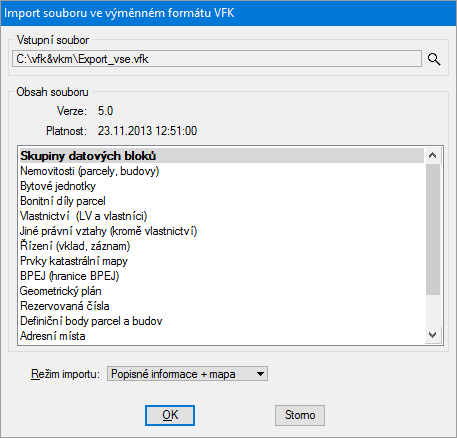
\includegraphics[height=9cm]{./pictures/gisoft.png}
      \caption{Ukázka načtení VFK dat (zdroj:
\href{http://www.gisoft.cz/cze/files/Moduly/import-vfk.png}{gisoft.cz})}
      \label{fig:gisoft}
  \end{figure}
%zdroj: http://www.gisoft.cz/Moduly/ImportVFK
%obrazek: http://www.gisoft.cz/cze/files/Moduly/import-vfk.png
\subsection{Spirit VFK}
Samospustitelná desktopová aplikace určená pro převod dat katastru
nemovitostí do libovolné geodatabáze ESRI. Do geodatabáze jsou
importovány tabulky, relace a ostatní databázové objekty
\zk{ISKN}. Výslednou databázi lze použít pro analytickou práci na
datech katastru nemovitostí nebo v aplikačních nadstavbách
\textit{Spirit KN} a~\textit{Spirit Portál}-KN. Produkt je od
společnosti GEOREAL s.r.o. a je zpoplatněný. Po krátké registraci je
možné vyzkoušet 30-ti denní Trial
verzi \footnote{http://mapy.georeal.cz/trialreg/}.\cite{spirit_vfk}
%zdroj: http://www.georeal.cz/cz/spirit-desktop/spirit-vfk
\subsection{TopoL xT}
TopoL xT je zpoplatněný software od společnosti TopoL. Je to obecný
geografický systém určený pro přípravu, správu a analýzu geografických
dat. Soubory výměnného formátu katastru nemovitostí (\zk{VFK}) jsou
jedním z podporovaných formátu při importu. Pro vyzkoušení je k
dispozici demonstrační
verze\footnote{http://www.topol.eu/files/download/topol/100/setup.exe},
ve které je omezený počet objektů, omezená velikost rastru a nelze
tisknout v měřítku.\citep{topol}

\begin{figure}[H]
	 \centering
      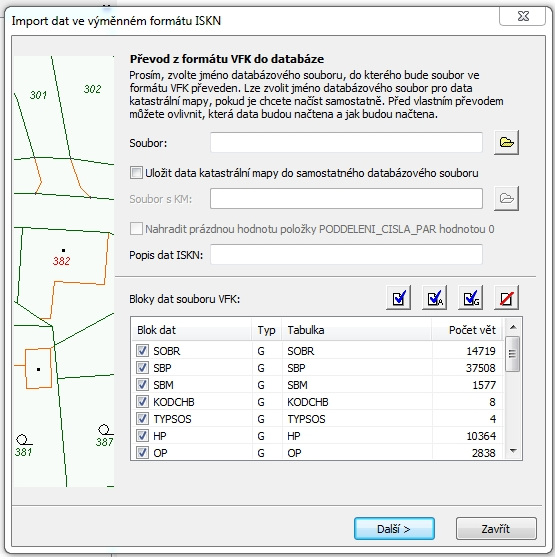
\includegraphics[height=9cm]{./pictures/topol.png}
      \caption{Ukázka importu VFK dat v programu TopoL xT (zdroj: vlastní)}
      \label{fig:topol}
  \end{figure}
%http://www.topol.eu/articles/software#topol-xt
\subsection{Kokeš}
Interakční grafický systém Kokeš od firmy GEPRO s.r.o. je zaměřený na
obor geodézie a na geoinformační systémy. V systému je možné řešit
nejrůznější geodetické i konstrukční výpočty, vytvářet a aktualizovat
kresby map, vést popisné údaje k objektům a bodům mapy, digitalizovat
grafické podklady. Budování systému po základních a uživatelských
funkcích umožňuje postupný vývoj a jednoduché
ovládání. \cite{kokes_cvut}

Funkce import \zk{VFK} umožňuje importovat jednotlivé soubory, kdy vstupem je jeden nebo více souborů \zk{VFK} (nebo ZIP) a výsledkem je jedna databáze SPI a~výkresy katastrální mapy, orientační mapy, definičních bodů parcel a definičních bodů budov. %\citep{napoveda_kokes}

\begin{figure}[H]
	 \centering
      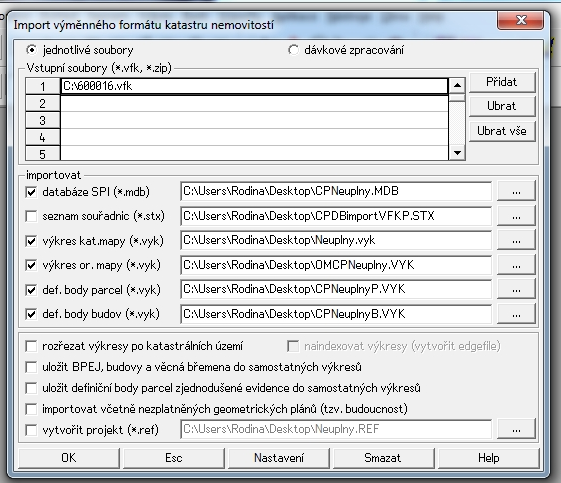
\includegraphics[width=10cm]{./pictures/kokes.png}
      \caption{Ukázka importu VFK dat v programu Kokeš (zdroj: vlastní)}
      \label{fig:kokes}
  \end{figure}
  
Informace o Funkci import \zk{VFK} pocházejí z nápovědy k funkci dostupné v samotném programu.
%zdroj: http://geo3.fsv.cvut.cz/~soukup/dip/bukovsky/1.htm, napoveda kokes k funkci import vfk
\subsection{ISKN Studio pro ArcGIS}
%% ML: dvakrat ve vete: formatu
Software určený pro import dat formátu \zk{ISKN} do formátu
%% ML: v predchazejim textu se spise objevuje VFK, ted mluvite o
%% NVF. Nikde neni zmineno, ze si pod zkratkou VFK predstavujete prave
%% NVF
geodatabáze. Pracuje s daty ve formátu NVF a umožňuje jejich
zpracování do osobní, souborové a ArcSDE geodatabáze v MS SQL Server
či Oracle. K ISKN Studiu je možné doinstalovat doplněk ISKN View,
který slouží k rychlému a jednoduchému vyhledávání v datech ISKN
převedených pomocí softwaru ISKN Studio. Jedná se o zpoplatněný
software. \cite{arcgis}

\begin{figure}[H]
	 \centering
      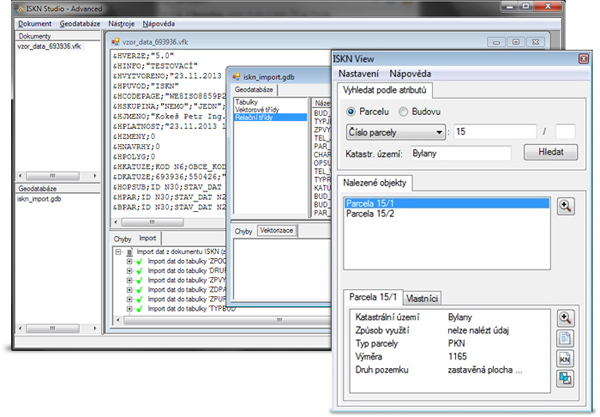
\includegraphics[height=9cm]{./pictures/iskn_studio.jpeg}
      \caption{Ukázka načtení VFK dat v ISKN Studiu (zdroj:
\href{https://www.arcdata.cz/uploads/media/general/0001/01/68f0bfd90cf19d903a57fc8457e1f228a7dd47f4.jpeg}{arcdata.cz})}
      \label{fig:ISKNStudio}
  \end{figure}
%zdroj:https://www.arcdata.cz/produkty/software-arcdata/import-iskn
%obrázek: https://www.arcdata.cz/uploads/media/general/0001/01/68f0bfd90cf19d903a57fc8457e1f228a7dd47f4.jpeg
\subsection{cadstudio}
V obou případech se jedná o konverzní aplikaci firmy CAD Studio
určenou pro zpracování dat \zk{ISKN}.
\begin{itemize}[leftmargin=50pt]
\item VFK2DB -- import dat do relační databáze Oracle nebo MS SQL Server, samostatně spustitelný program \cite{vfk2db} %http://www.cadstudio.cz/vfk
\item VFK2DWG -- automatický převod souboru či souborů VFK přímo na objekty AutoCADu a nimi svázané databázové tabulky, nadstavba AutoCADu \cite{vfk2dwg}

\begin{figure}[H]
	 \centering
      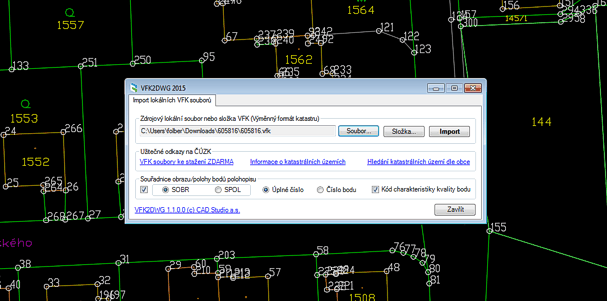
\includegraphics[width=14cm]{./pictures/vfk2dwg.png}
      \caption{Import VFK souborů (zdroj:
\href{http://www.cadstudio.cz/img/vfk2dwg11.gif}{cadstudio.cz})}
      \label{fig:cadstudio}
  \end{figure}
%http://www.cadstudio.cz/vfk2dwg
\end{itemize}
\subsection{Knihovna GDAL}
\label{subsec:gdal_vfk}
VFK Driver je součástí knihovny \zk{GDAL} a umožňuje čtení souborů
výměnného formátu katastru nemovitostí (VFK). Driver, česky ovladač,
slouží obecně k rozšíření funkcionality. Soubor \zk{VFK} je driverem
vnímán jako zdroj dat (\verb|OGR datasource|) s žádnou nebo více
vrstvami (\verb|OGR layers|). Body jsou ve vrstvách reprezentovány
jako \verb|wkbPoints|, linie a hranice jako \verb|wkbLineStrings| a
plochy jako \verb|wkbPolygons|. VFK driver si během prvního čtení
ukládá data do SQLite databáze, která se vytvoří ve stejném adresáři
jako je VFK soubor. Opakované načtení je díky již vytvořené databázi
výrazně rychlejší. Výhoda databáze je v snazším a rychlejším přístupu
k datům. Dále si může uživatel pomocí systémových proměnných
\verb|OGR_VFK_DB_OVERWRITE| a \verb|OGR_VFK_DB_NAME| nastavit, jestli
bude vytvořená SQLite databáze při opakovaném načtení přepsána (čtení
stále z VFK souboru) a jaký bude název vytvořené databáze. Navíc je
tento driver jako jediný z výše zmíněných nástrojů volně
dostupný. \cite{vfk_driver}

\begin{figure}[H]
	 \centering
      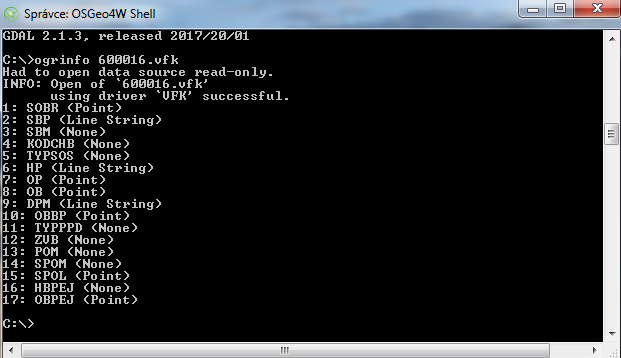
\includegraphics[width=15cm]{./pictures/vfk_driver.png}
      \caption{Ukázka použití VFK driveru (zdroj:vlastní)}
      \label{fig:vfk_driver}
  \end{figure}
%zdroj:http://gdal.org/drv_vfk.html
%http://freegis.fsv.cvut.cz/gwiki/VFK_/_GDAL
%http://freegis.fsv.cvut.cz/gwiki/V%C3%BDm%C4%9Bnn%C3%BD_form%C3%A1t_ISKN
%VFK/QGIS plugin
%http://freegis.fsv.cvut.cz/gwiki/VFK_/_QGIS_plugin
\section{Sestavení geometrie prvků}
\label{sec:sestaveni_geometrie}
Po načtení \zk{VFK} souboru knihovnou GDAL (viz \ref{subsec:gdal_vfk})
nedojde k sestavení geometrie prvků automaticky, pokud je verze
knihovny GDAL 2.1 a nižší. Uživatel si proto musí o sestavení
%% ML: ve vete se trikrat opakuje slovo ``geometrie''
geometrie sám říct dotazem na požadovanou geometrii, například
chceme-li geometrii bloku HP:
\textbf{GetLayerByName('HP').GetFeature(1)}. Geo\-metrie se sestavuje
postupně po blocích dle schématu počínaje blokem SOBR (souřadnice
%% ML: misto dvojtecky, uvedte odkaz na obrazek
obrazu bodů polohopisu):
\begin{figure}[H]
	 \centering
      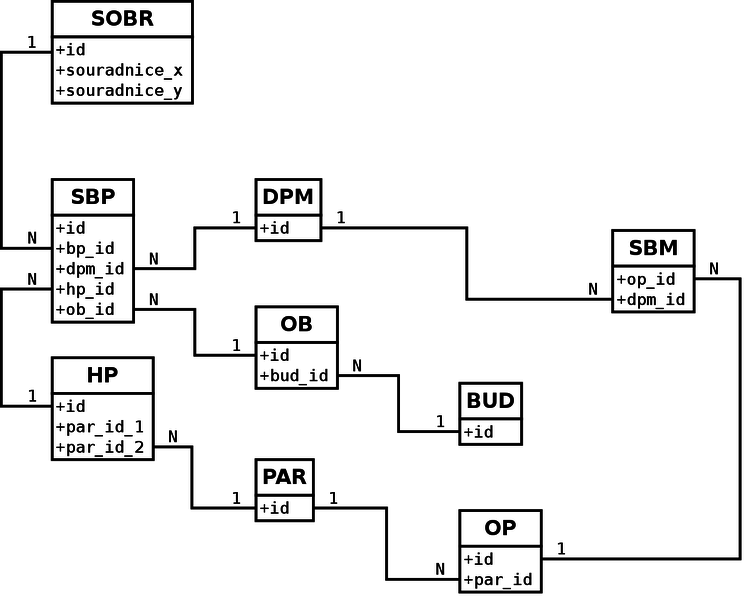
\includegraphics[width=10cm]{./pictures/Vfk-diagram-geom.png}
      \caption{Přehled datových bloků pro sestavení geometrie prvků digitální katastrální mapy (zdroj:
      \href{http://freegis.fsv.cvut.cz/wiki/images/thumb/8/8a/Vfk-diagram-geom.png/744px-Vfk-diagram-geom.png}{freegis.fsv.cvut.cz})}
      \label{fig:vfk_diagram_geom}
\end{figure}
%% ML: vetu prepiste, zni kostrbate
Pokud má být sestavena geometrie bloku HP (hranic parcel), dojde po
provedení dotazu na geometrii hranic parcel k sestavení geometrie i
%% ML: predchozich -> souvisejicich
všech předchozích bloků. Výsledkem dotazu je tedy sestavená geometrie
nejen pro blok hranic parcel, ale také pro blok SOBR (souřadnice
obrazu bodů polohopisu) a blok SBP (spojení bodů
polohopisu). Geometrie datového bloku HP je pro tuto práci důležitá,
%% ML: sestaveni geometrie?
protože právě z ní dojde k sestavení bloku PAR (parcely). Stejně tak
datový blok SBP, který bude využit k sestavení bloku BUD (budovy).
%zdroj: http://freegis.fsv.cvut.cz/gwiki/VFK_/_GDAL
